\subsection{Conexión de dispositivos finales}

Tendremos dos casos en cuando se quieran conectar dos o más dispositivos finales, el primero es cuando es posible que se comuniquen entre si por que tienen direcciones IP ruteables.
El segundo caso es cuando los dispositivos finales no pueden comunicarse entre si por que no tienen direcciones IP ruteables, en este caso el orquestrador deberá ofrecer un mecanismo para que los dispositivos finales puedan conectarse entre sí mediante un relay.
\begin{figure}[h!]
    \centering
    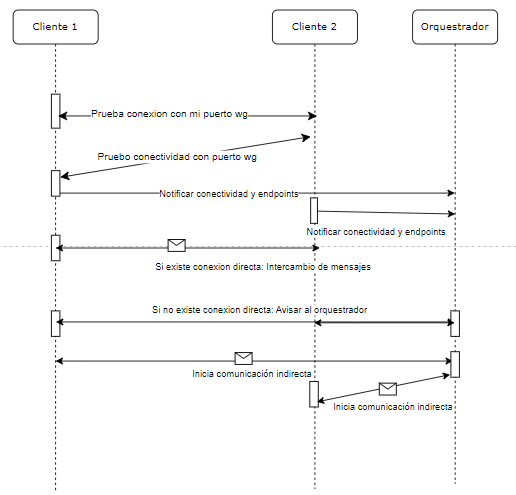
\includegraphics[width=\textwidth]{alcanzabilidad.png}
    \caption{Diagrama de caso de uso: conexión de dispositivos finales}
\end{figure}

\subsubsection{Conexión de dispositivos finales con direcciones IP ruteables. Directa}

En este caso el uno de los clientes se comunica directamente con el otro cliente, el orquestrador deberá enviar un mensaje de confirmación al cliente que solicita la conexión. 
Para esto el cliente A enviara mediante ping al cliente B a la dirección IP y puerto que el orquestrador le proporcionó para la interfaz Wireguard.

Si se obtiene una respuesta entonces consideramos que la conexión fue exitosa (los dispositivos son alcanzables). 
\begin{figure}[h!]
    \centering
    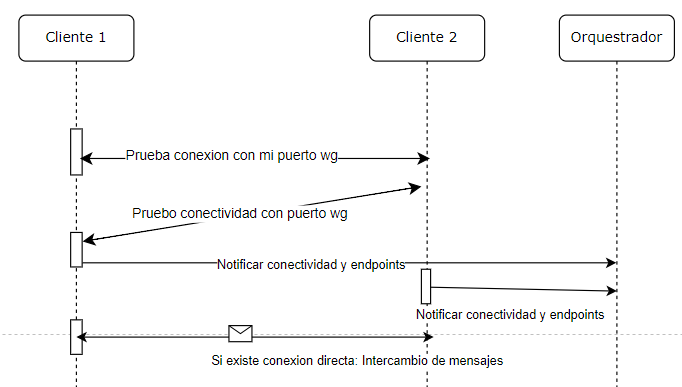
\includegraphics[width=\textwidth]{conexion-directa.png}
    \caption{Diagrama de caso de uso: conexión de dispositivos finales con direcciones IP ruteables. Directa}
\end{figure}


\subsubsection{Conexión de dispositivos finales con direcciones IP no ruteables. Relay}

En este caso el orquestrador deberá ofrecer un mecanismo para que los dispositivos finales puedan conectarse entre sí mediante un relay. 
El cliente A se comunica con el orquestrador para solicitar la conexión con el cliente B, el orquestrador deberá enviar un mensaje de confirmación al cliente A con la dirección IP y puerto del orquestrador, el cliente A deberá enviar un mensaje al orquestrador para que este se comunique con el cliente B. 

\begin{figure}[h!]
    \centering
    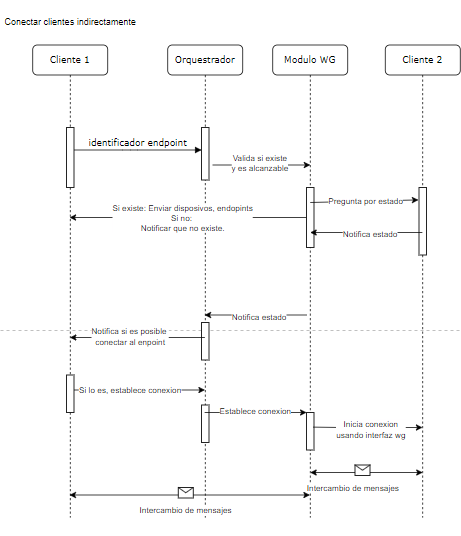
\includegraphics[width=\textwidth]{conecta-clientes-indirectamente.png}
    \caption{Diagrama de caso de uso: conexión de dispositivos finales con direcciones IP no ruteables. Relay}
\end{figure}